
\section{Per-fold homology leakage audit}\label{app:homology}
Random stratified cross-validation does not control homology between the
training and held-out partitions. For each fold of the study-14 protocol we
count held-out sequences sharing at least one exact contiguous decamer
($k{=}10$) with any training sequence (the union-find criterion of
Definition~\ref{def:cluster} restricted to train--test pairs).

\begin{table}[h]\centering\small
\caption{Held-out sequences sharing an exact decamer with the training
partition, per fold of the Feb2020 10-fold CV.}
\label{tab:homologyfolds}
\begin{tabular}{cccc}
\hline
Fold & Held-out $n$ & Sharing a decamer & Fraction (\%) \\
\hline
1 & 405 & 61 & 15.06 \\
2 & 405 & 64 & 15.80 \\
3 & 404 & 50 & 12.38 \\
4 & 404 & 70 & 17.33 \\
5 & 404 & 57 & 14.11 \\
6 & 404 & 86 & 21.29 \\
7 & 404 & 53 & 13.12 \\
8 & 404 & 68 & 16.83 \\
9 & 404 & 65 & 16.09 \\
10 & 404 & 72 & 17.82 \\
\hline
\multicolumn{4}{l}{overall: 15.98\% of all held-out sequences} \\
\end{tabular}
\end{table}

Roughly one in six held-out sequences is decamer-redundant with training,
so the random-CV numbers of Table~\ref{tab:feb2020} overstate performance
on genuinely remote sequences. A cluster-held-out variant of the same
protocol is the correct control and is recorded as future work; the
cluster-aware split of our own large dataset
(Section~\ref{sec:labelconfound}) shows the direction and size of the drop
such control induces.

\begin{figure}[h]\centering
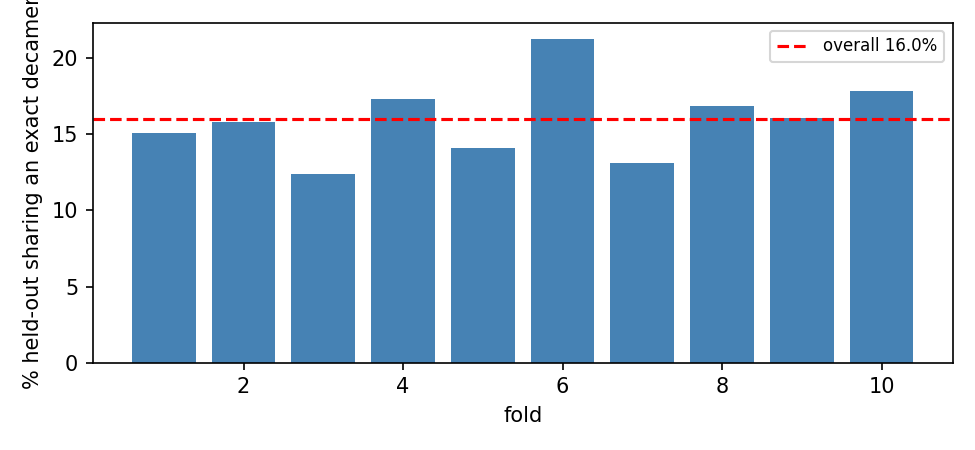
\includegraphics[width=0.75\textwidth]{fig_homology_folds.png}
\caption{Per-fold fraction of held-out sequences sharing an exact decamer
with the training partition (study 16).}
\label{fig:homologyfolds}
\end{figure}
